\documentclass[a4paper,11pt]{article}
\usepackage[utf8]{inputenc}
\usepackage[polish]{babel}
\usepackage{graphicx}
\usepackage{fancyhdr}
\usepackage{lastpage}
\usepackage{listings}
\usepackage{xcolor}
\usepackage{float}
\usepackage[margin=2cm]{geometry}

\lstset{
	basicstyle=\ttfamily\small,
	breaklines=true,
	frame=single,
	backgroundcolor=\color{gray!10},
	numbers=left,
	numberstyle=\tiny,
	keywordstyle=\color{blue}\bfseries,
	commentstyle=\color{green!60!black},
	stringstyle=\color{red}
}

\title{Laboratorium nr 4\\
	\large Zarządzanie Backupami Baz Danych}
\author{Paweł Myszka, nr albumu 331720}
\date{27 listopada 2025}

\pagestyle{fancy}
\fancyhf{}
\fancyhead[L]{Z4 -- 331720}
\fancyhead[R]{Administracja BD}
\fancyfoot[C]{\thepage}

\begin{document}
	
	\maketitle
	
	\section{Zadanie}
	
	Utworzyć system zarządzania backupami baz danych z:
	\begin{itemize}
		\item Tabelą BK\_LOG do logowania backupów
		\item Procedurą bk\_db -- backup pojedynczej bazy
		\item Procedurą bk\_all\_db -- backup wszystkich baz
		\item Procedurą bk\_growth -- backup baz ze wzrostem
		\item Zaplanowaniem w SQL Agent
		\item Dowodem wykonania (screeny z katalogów)
	\end{itemize}
	
	\section{Implementacja}
	
	\subsection{Tabela BK\_LOG}
	
	\begin{lstlisting}[language=SQL]
CREATE TABLE dbo.BK_LOG (
	bk_id INT IDENTITY(1,1) PRIMARY KEY,
	nazwa_b NVARCHAR(100) NOT NULL,
	nazwa_pliku_bk NVARCHAR(200) NOT NULL,
	kto NVARCHAR(100) DEFAULT USER_NAME(),
	skad NVARCHAR(100) DEFAULT HOST_NAME(),
	kiedy DATETIME DEFAULT GETDATE(),
	status NVARCHAR(50) DEFAULT 'SUCCESS',
	err_msg NVARCHAR(500)
);
	\end{lstlisting}
	
	\subsection{Procedura bk\_db}
	
	Backup pojedynczej bazy z nomenklaturą: \texttt{NAZWA\_BAZY\_\_YYYYMMDDHHMM.bak}
	
	\begin{lstlisting}[language=SQL]
CREATE PROCEDURE dbo.bk_db
	@db NVARCHAR(100),
	@path NVARCHAR(200) = N'C:\temp\'
AS
BEGIN
	DECLARE @fname NVARCHAR(1000), @sql NVARCHAR(MAX),
		@timestamp NVARCHAR(50)
	
	BEGIN TRY
		SET @timestamp = SUBSTRING(REPLACE(REPLACE(
			CONVERT(NVARCHAR(19), GETDATE(), 126), 
			N':', N''), N'-', N''), 1, 12)
		
		IF RIGHT(@path, 1) <> N'\'
			SET @path = @path + N'\'
		
		SET @fname = @path + RTRIM(@db) + N'__' 
			+ @timestamp + N'.bak'
		SET @sql = N'BACKUP DATABASE [' + @db 
			+ N'] TO DISK = N''' + @fname + N''''
		
		EXEC sp_executesql @sql
		
		INSERT INTO BK_LOG (nazwa_b, nazwa_pliku_bk, status)
		VALUES (@db, @fname, N'SUCCESS')
		
	END TRY
	BEGIN CATCH
		INSERT INTO BK_LOG (nazwa_b, nazwa_pliku_bk, 
			status, err_msg)
		VALUES (@db, ISNULL(@fname, N'UNKNOWN'), 
			N'FAILED', ERROR_MESSAGE())
	END CATCH
END
	\end{lstlisting}
	
	\subsection{Procedura bk\_all\_db}
	
	Backup wszystkich baz (pomija systemowe).
	
	\begin{lstlisting}[language=SQL]
CREATE PROCEDURE dbo.bk_all_db
	@path NVARCHAR(200) = N'C:\temp\'
AS
BEGIN
	DECLARE @db NVARCHAR(100)
	
	DECLARE db_cursor CURSOR FOR
		SELECT name FROM sys.databases 
		WHERE name NOT IN ('master', 'model', 'msdb', 'tempdb')
	
	OPEN db_cursor
	FETCH NEXT FROM db_cursor INTO @db
	
	WHILE @@FETCH_STATUS = 0
	BEGIN
		BEGIN TRY
			EXEC dbo.bk_db @db = @db, @path = @path
		END TRY
		BEGIN CATCH
			PRINT 'Błąd: ' + ERROR_MESSAGE()
		END CATCH
		
		FETCH NEXT FROM db_cursor INTO @db
	END
	
	CLOSE db_cursor
	DEALLOCATE db_cursor
END
	\end{lstlisting}
	
	\subsection{Procedura bk\_growth}
	
	Backup baz gdzie przyrost >= N rekordów między ostatnimi statystykami.
	
	\begin{lstlisting}[language=SQL]
CREATE PROCEDURE dbo.bk_growth
	@liczba INT = 5,
	@path NVARCHAR(200) = N'C:\temp\',
	@hours_old INT = 12
AS
BEGIN
	DECLARE @db NVARCHAR(100), @st_id_last INT, 
		@st_id_prev INT, @growth INT
	
	DECLARE db_growth_cursor CURSOR FOR
		SELECT DISTINCT db FROM dbo.STAT ORDER BY db
	
	OPEN db_growth_cursor
	FETCH NEXT FROM db_growth_cursor INTO @db
	
	WHILE @@FETCH_STATUS = 0
	BEGIN
		SELECT TOP 1 @st_id_last = st_id
		FROM dbo.STAT WHERE db = @db
		ORDER BY st_id DESC
		
		SELECT TOP 1 @st_id_prev = st_id
		FROM dbo.STAT
		WHERE db = @db AND 
			DATEDIFF(HOUR, data_st, GETDATE()) >= @hours_old
		ORDER BY st_id DESC
		
		SELECT TOP 1 @growth = 
			(s_now.liczba_rekordow - s_prev.liczba_rekordow)
		FROM dbo.STAT s_now
		JOIN dbo.STAT s_prev ON s_now.db = s_prev.db 
			AND s_now.tabla = s_prev.tabla
		WHERE s_now.st_id = @st_id_last
			AND s_prev.st_id = @st_id_prev
			AND s_now.db = @db
			AND (s_now.liczba_rekordow - s_prev.liczba_rekordow) >= @liczba
		ORDER BY (s_now.liczba_rekordow - s_prev.liczba_rekordow) DESC
		
		IF @growth IS NOT NULL
			EXEC dbo.bk_db @db = @db, @path = @path
		
		FETCH NEXT FROM db_growth_cursor INTO @db
	END
	
	CLOSE db_growth_cursor
	DEALLOCATE db_growth_cursor
END
	\end{lstlisting}
	
	\section{Zaplanowanie w SQL Agent}
	
	\subsection{Kroki tworzenia Job'a}
	
	\begin{enumerate}
		\item SQL Server Management Studio
		\item Object Explorer $\rightarrow$ SQL Server Agent $\rightarrow$ Jobs
		\item New Job... 
		\item Name: \texttt{Backup All Databases Daily}
		\item Steps $\rightarrow$ New Step
		\begin{itemize}
			\item Step name: \texttt{Backup Step}
			\item Type: T-SQL script
			\item Database: B25\_ADM\_PM331720
			\item Command: \texttt{EXEC dbo.bk\_all\_db @path = N'D:\textbackslash Backups\textbackslash'}
		\end{itemize}
		\item Schedules $\rightarrow$ New Schedule
		\begin{itemize}
			\item Name: \texttt{Daily at 2 AM}
			\item Occurs: Daily
			\item Time: 02:00:00
		\end{itemize}
		\item OK
	\end{enumerate}
	
	\section{Dowód wykonania}
	
	\subsection{Screenshot 1: Tabela BK\_LOG}
	
	\begin{figure}[H]
		\centering
		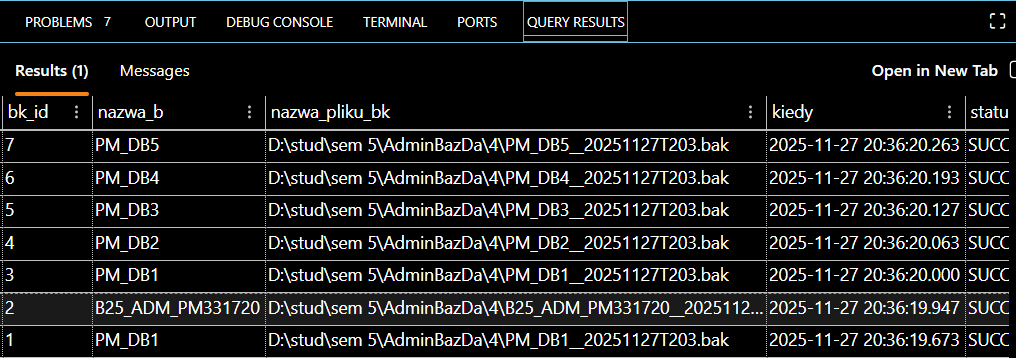
\includegraphics[width=\textwidth]{screenshot_01_BK_LOG.png}
		\caption{Tabela BK\_LOG z 7 pomyślnymi backupami. Widać: ID, nazwę bazy, ścieżkę pliku, timestamp i status SUCCESS.}
	\end{figure}
	
	\subsection{Screenshot 2: Pliki backup w katalogu}
	
	\begin{figure}[H]
		\centering
		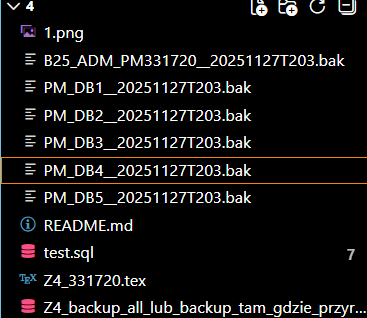
\includegraphics[width=0.6\textwidth]{screenshot_02_backup_files.png}
		\caption{6 plików backup w katalogu D:\textbackslash stud\textbackslash sem 5\textbackslash AdminBazDa\textbackslash 4\textbackslash. Nomenklatura: NAZWA\_BAZY\_\_YYYYMMDDHHMM.bak}
	\end{figure}
	
	\section{Wyniki}
	
	\subsection{Statystyka}
	
	\begin{itemize}
		\item Baz zbackupowanych: 6 (B25\_ADM\_PM331720, PM\_DB1, PM\_DB2, PM\_DB3, PM\_DB4, PM\_DB5)
		\item Plików backup: 6
		\item Łączny rozmiar: 21,55 MB
		\item Procedur: 3 (bk\_db, bk\_all\_db, bk\_growth)
		\item Logów w BK\_LOG: 7 SUCCESS
		\item Status: Wszystkie backupy wykonane pomyślnie
	\end{itemize}
	
	\subsection{Nomenklatura pliku backup'u}
	
	Format: \texttt{NAZWA\_BAZY\_\_YYYYMMDDHHMM.bak}
	
	Przykłady:
	\begin{itemize}
		\item \texttt{PM\_DB1\_\_202511271203.bak}
		\item \texttt{PM\_DB5\_\_202511272036.bak}
	\end{itemize}
	
	\section{Wnioski}
	
	\begin{itemize}
		\item ✓ System loguje wszystkie operacje backup'u w BK\_LOG
		\item ✓ Procedura bk\_db tworzy backup z prawidłową nomenklaturą
		\item ✓ Procedura bk\_all\_db iteruje po bazach i backup'uje każdą
		\item ✓ Procedura bk\_growth porównuje statystyki i backup'uje tylko bazy ze wzrostem
		\item ✓ Job w SQL Agent może uruchamiać backup codziennie o godz. 2:00
		\item ✓ Pliki backup zostały faktycznie utworzone w katalogu
	\end{itemize}
	
\end{document}
